\documentclass[letterpaper,12pt]{article}
\usepackage{tabularx} % extra features for tabular environment
\usepackage{amsmath}  % improve math presentation
\usepackage{float}
\usepackage{pdfpages}
\usepackage{steinmetz}

\usepackage{graphicx} % takes care of graphic including machinery
\graphicspath{ {./figures/} }
\usepackage[margin=1in,letterpaper]{geometry} % decreases margins
\usepackage{cite} % takes care of citations
\usepackage[final]{hyperref} % adds hyper links inside the generated pdf file
\hypersetup{
	colorlinks=true,       % false: boxed links; true: colored links
	linkcolor=blue,        % color of internal links
	citecolor=blue,        % color of links to bibliography
	filecolor=magenta,     % color of file links
	urlcolor =blue         
}




\begin{document}

\title{Experiment 5 Preliminary Work \protect\\ Bipolar Junction Transistor Characteristics}
\author{Ahmet Akman 2442366 \protect\\}
\date{\today}
\maketitle
\tableofcontents
%\begin{abstract}
%abstract
%\end{abstract}

%\section{Introduction}
\section{Step 1}
The document entitled "Notes on Transistors" is read.
\section{Step 2}
One can check whether the a known transistor is defective or not by connecting the probes of the multimeter to the p--->n directions of the transistor . So that if the pn junction is operating one can say transistor is not defective. On the other hand given an unknown transistors is not defective one can determine whether it is npn or pnp by the same featre of the multimeter.
\section{Step 3}
\begin{table}[H]
    \begin{center}
        \caption{Resistance reading by color code convention.}
        \vspace{2mm}
        \begin{tabular}{||c | c | c||} 
            \hline
             & C547-B & C557-B \\ [0.5ex] 
            \hline\hline
            Collector Emitter Voltage (V) & 45 &-45  \\ 
            \hline
            Collector Base Voltage (V)   & 50 & -50   \\
            \hline
            Emitter Base Voltage (V) & 60 & -5  \\  
            \hline
            
            Collector Current(A) & 100mA & -100mA\\ 
            \hline
            
            \(\beta\) & 110-800 & 120-800  \\ 
             
            \hline
            Temperature Range (Celcius) & -55 to 150 C & -55 to 150 C \\ [1ex] 
            \hline
        \end{tabular}
    \end{center}
    \end{table}



\section{Step 4}
The expected plot can be illustrated as given in Figure 1.
\begin{figure}[H]
    \centering
    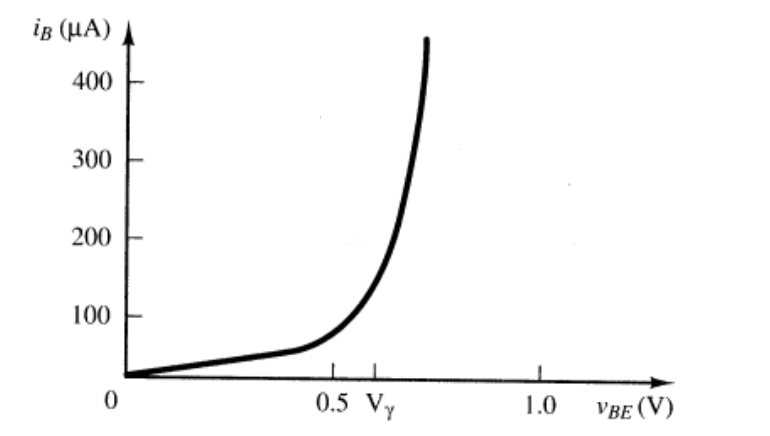
\includegraphics[width=1\textwidth]{4a.png}
    \caption{Expected plot (borrowed from the notes on transistors)}
    \end{figure} 
\section{Step 5}
\section{Step 6}
\section{Step 7}
\subsection{a.}
For this part the simulation is done with the reference circuit given in Figure 2.
\begin{figure}[H]
    \centering
    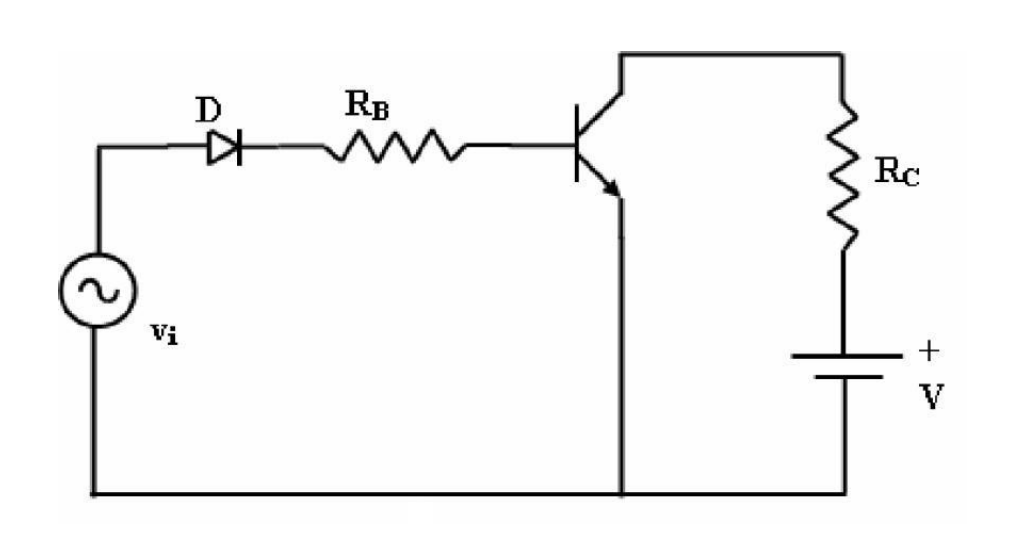
\includegraphics[width=1\textwidth]{fig1.png}
    \caption{Circuit schematic for the step 7 a}
    \end{figure} 
    The circuit given in Figure 3 is constructed in LTSpice simulation environment.
\begin{figure}[H]
\centering
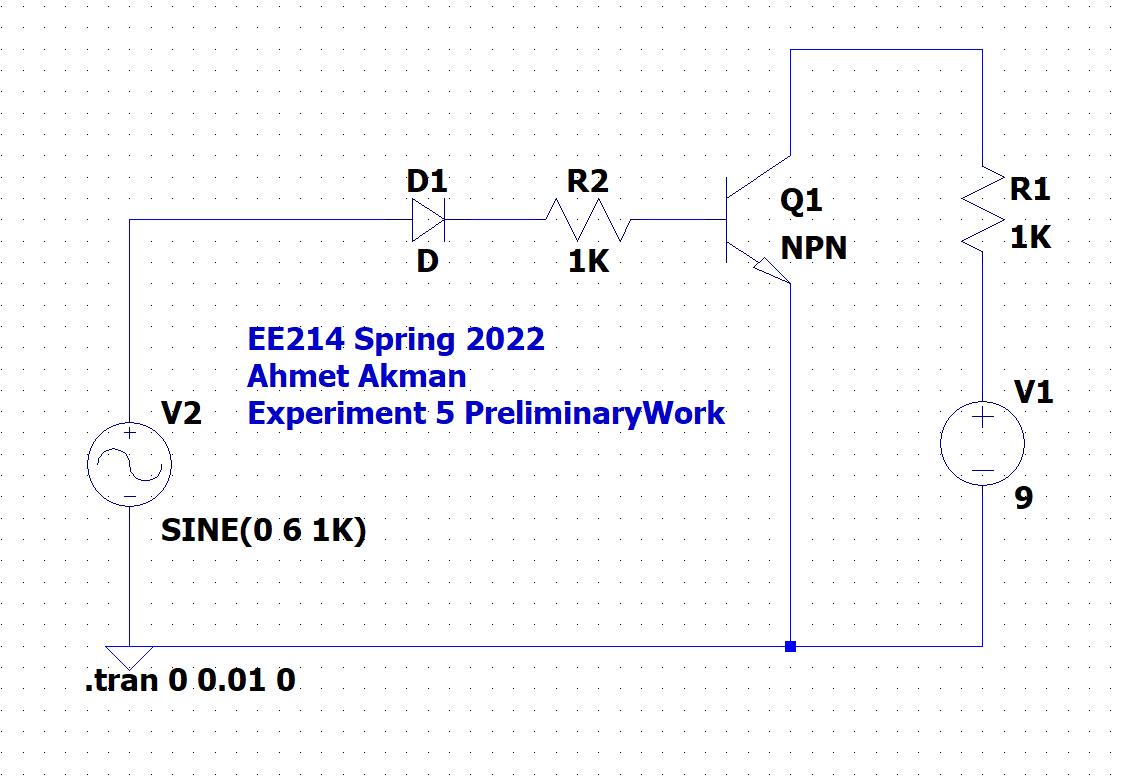
\includegraphics[width=1\textwidth]{1sim.png}
\caption{Circuit simulation schematic for the step 7 a}
\end{figure} 
As a result plot given in Figure 4 is obtained.
\begin{figure}[H]
    \centering
    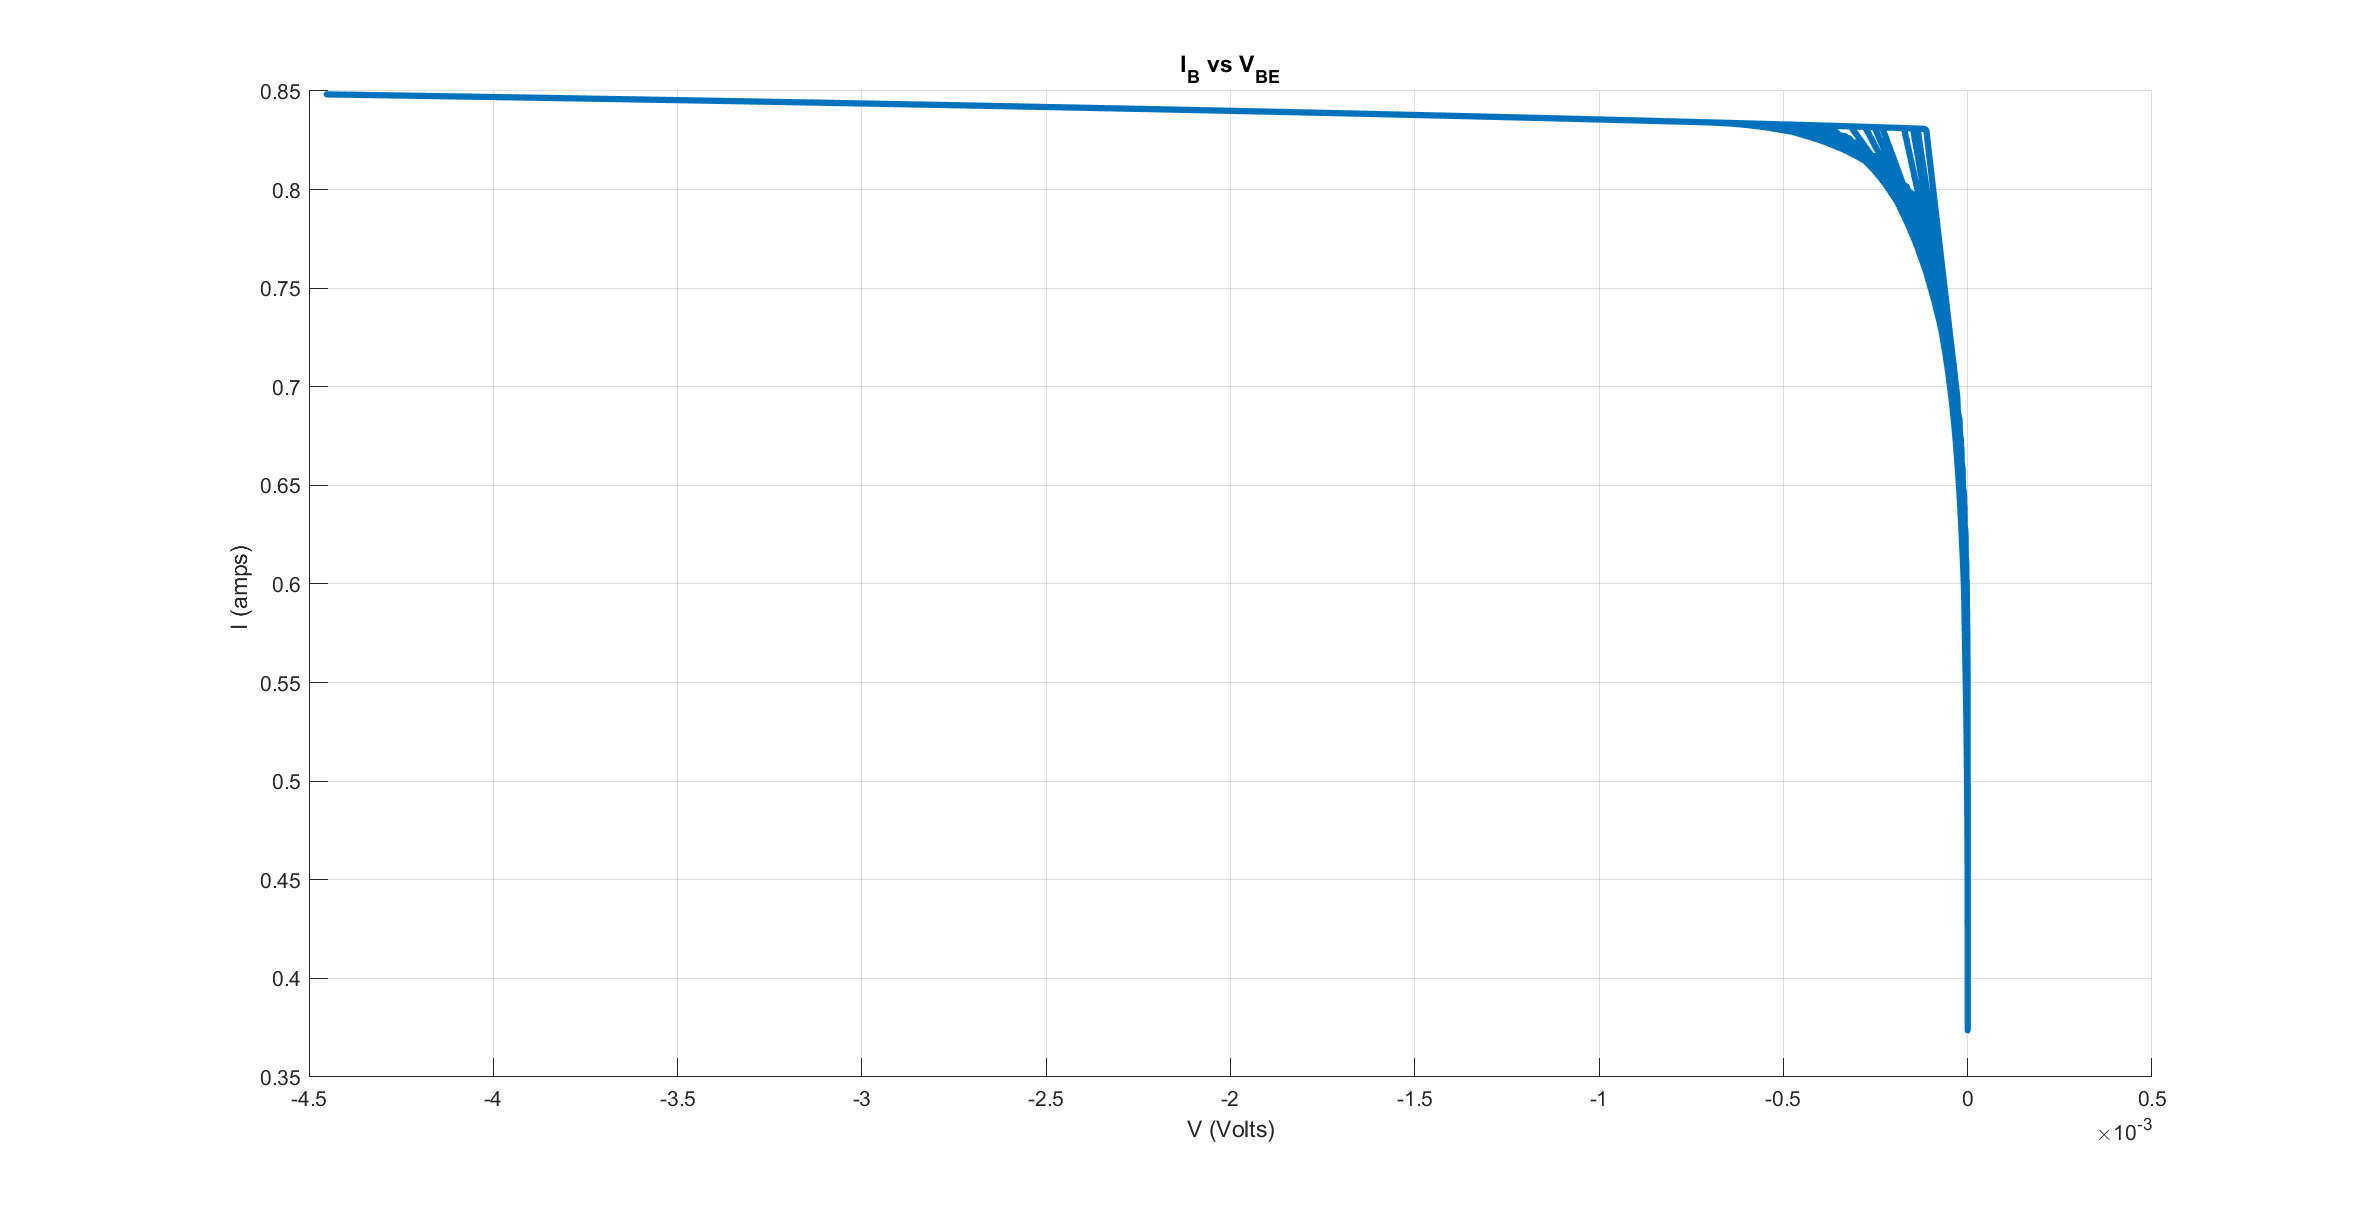
\includegraphics[width=1\textwidth]{7_1.png}
    \caption{Plot for step 7 a}
    \end{figure} 
    
\subsection{b.}
For this part the simulation is done with the reference circuit given in Figure 5.
\begin{figure}[H]
    \centering
    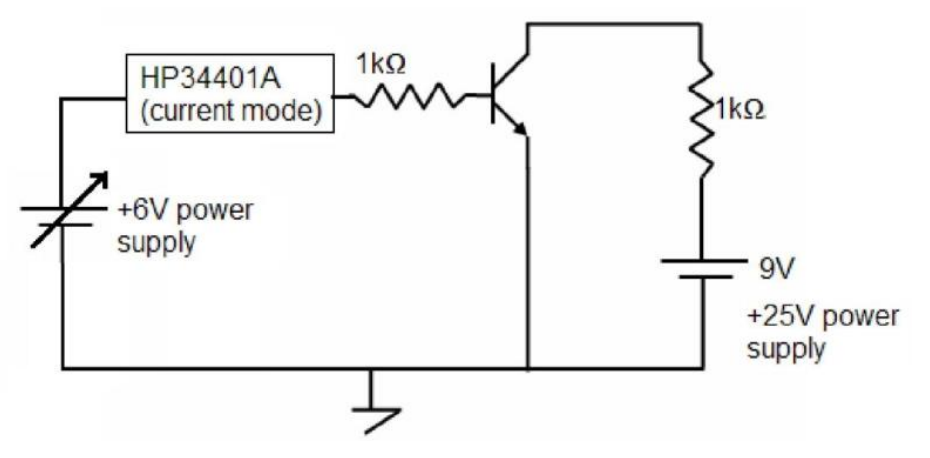
\includegraphics[width=1\textwidth]{fig5.png}
    \caption{Circuit schematic for the step 7 b}
    \end{figure} 
    The circuit given in Figure 6 is constructed in LTSpice simulation environment.
\begin{figure}[H]
\centering
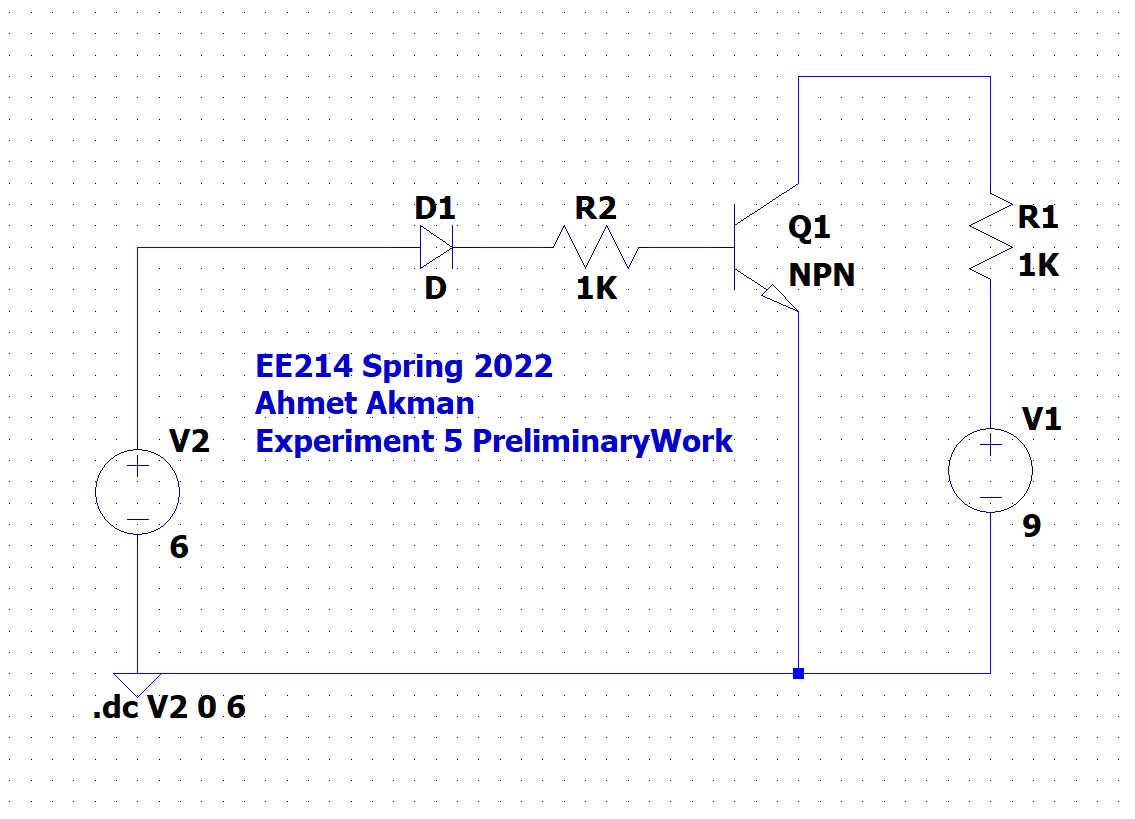
\includegraphics[width=1\textwidth]{5sim.png}
\caption{Circuit simulation schematic for the step 7 b}
\end{figure} 
As a result plot given in Figure 7 is obtained.
\begin{figure}[H]
    \centering
    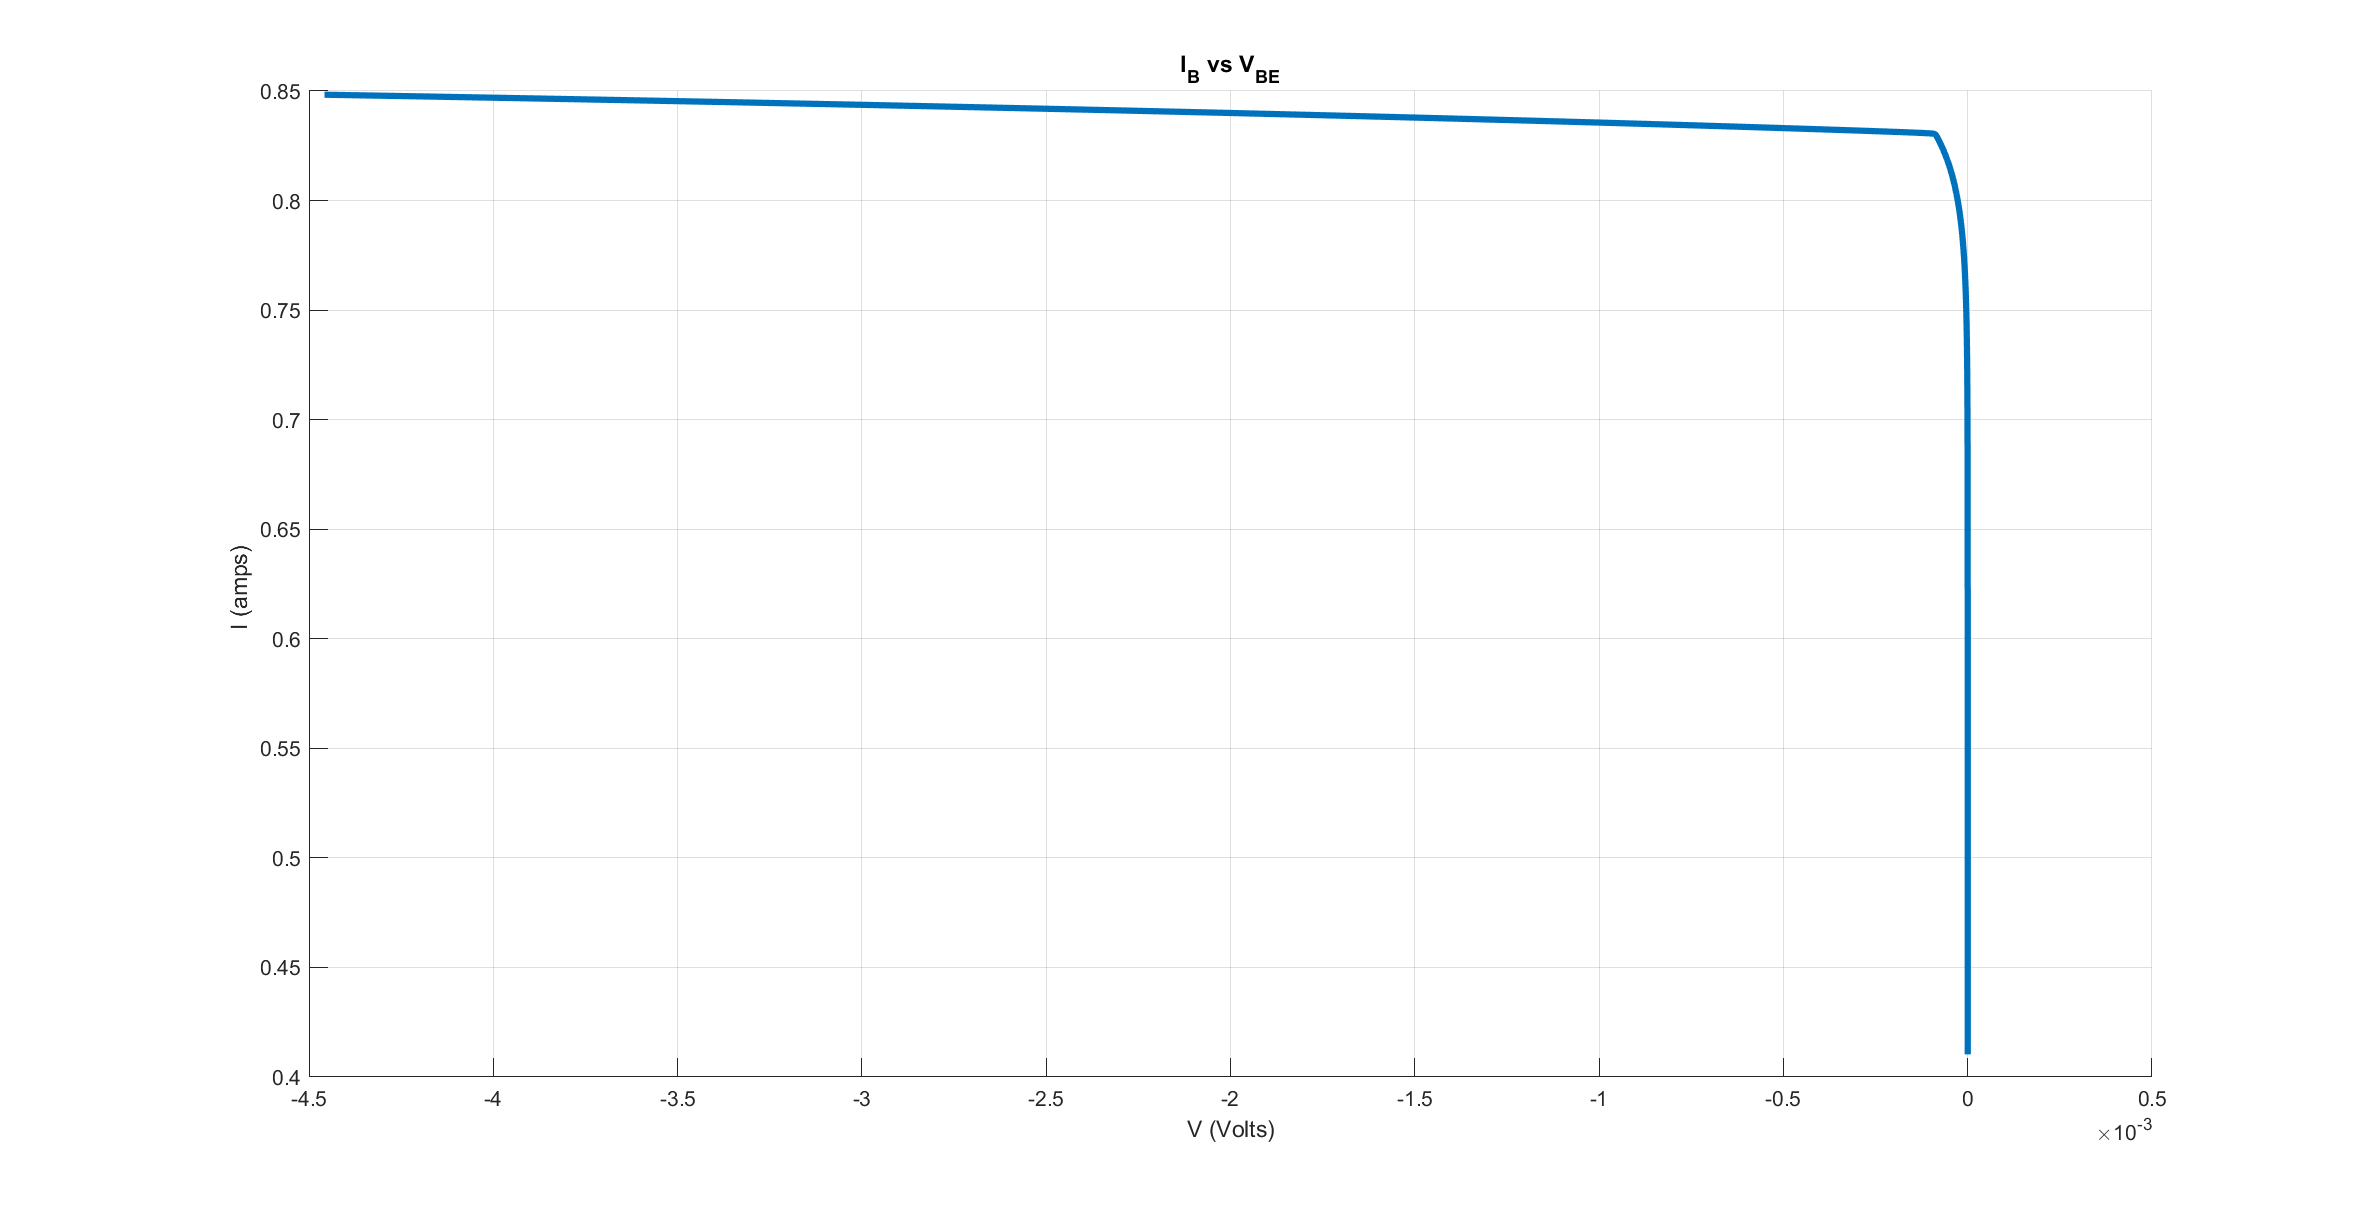
\includegraphics[width=1\textwidth]{7_2.png}
\caption{Plot for step 7 a}
\end{figure} 
\subsection{c.}
For this part the simulation is done with the reference circuit given in Figure 8.
\begin{figure}[H]
    \centering
    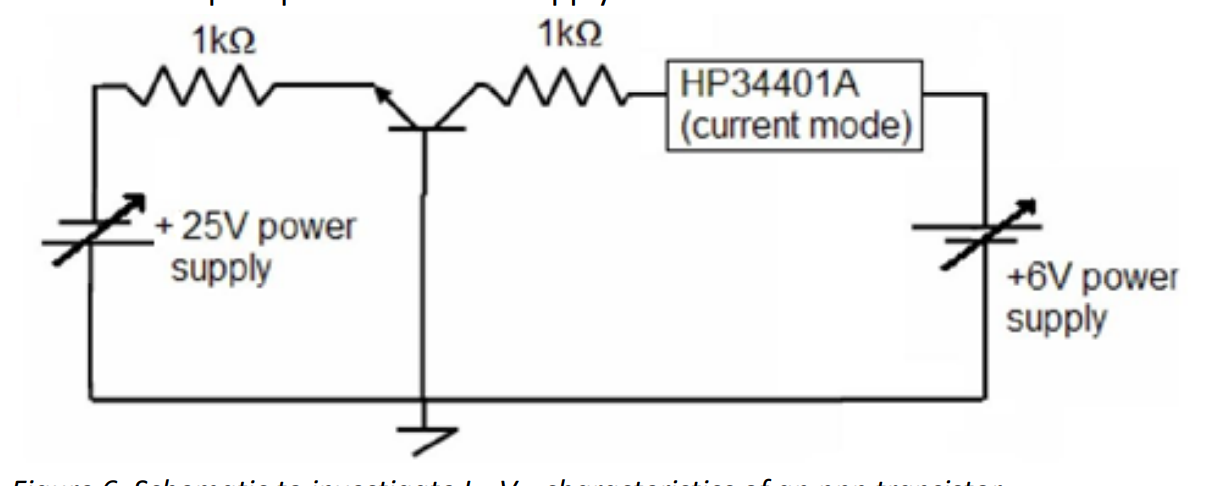
\includegraphics[width=1\textwidth]{fig6.png}
    \caption{Circuit schematic for the step 7 c}
    \end{figure} 
    The circuit given in Figure 9 is constructed in LTSpice simulation environment.
\begin{figure}[H]
\centering
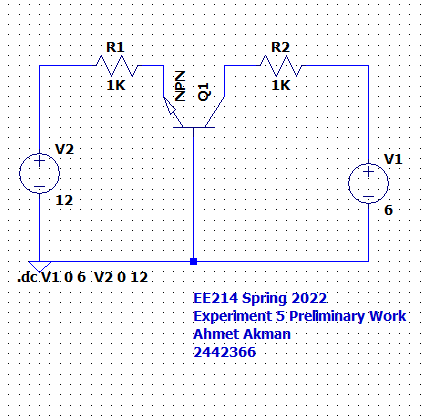
\includegraphics[width=1\textwidth]{6sim.png}
\caption{Circuit simulation schematic for the step 7 c}
\end{figure} 
As a result plot given in Figure 10 is obtained.
\begin{figure}[H]
    \centering
    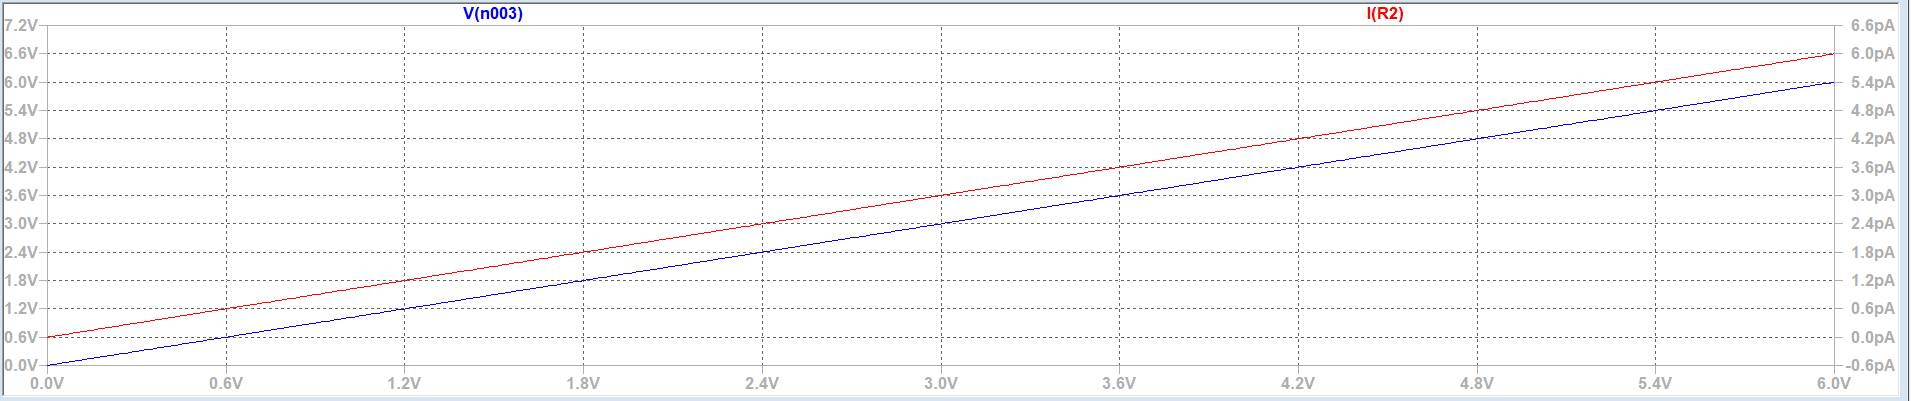
\includegraphics[width=1\textwidth]{7_d_plot.png}
\caption{Plot for step 7 c}
\end{figure} 

\subsection{d.}

For this part the simulation is done with the reference circuit given in Figure 11.
\begin{figure}[H]
    \centering
    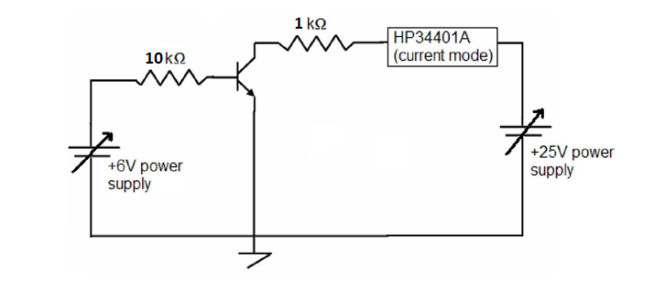
\includegraphics[width=1\textwidth]{fig7.png}
    \caption{Circuit schematic for the step 7 d}
    \end{figure} 
    The circuit given in Figure 12 is constructed in LTSpice simulation environment.
\begin{figure}[H]
\centering
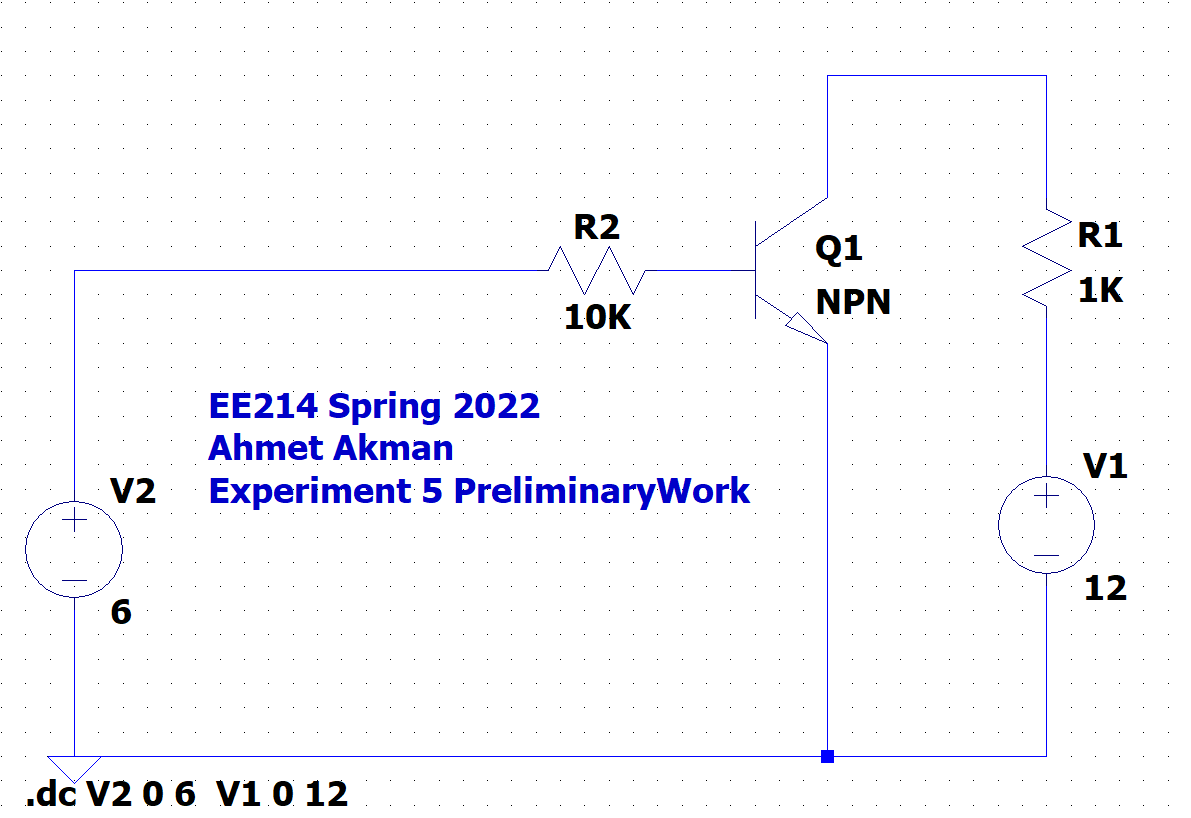
\includegraphics[width=1\textwidth]{7sim.png}
\caption{Circuit simulation schematic for the step 7 d}
\end{figure} 
As a result plot given in Figure 13 is obtained.
\begin{figure}[H]
    \centering
    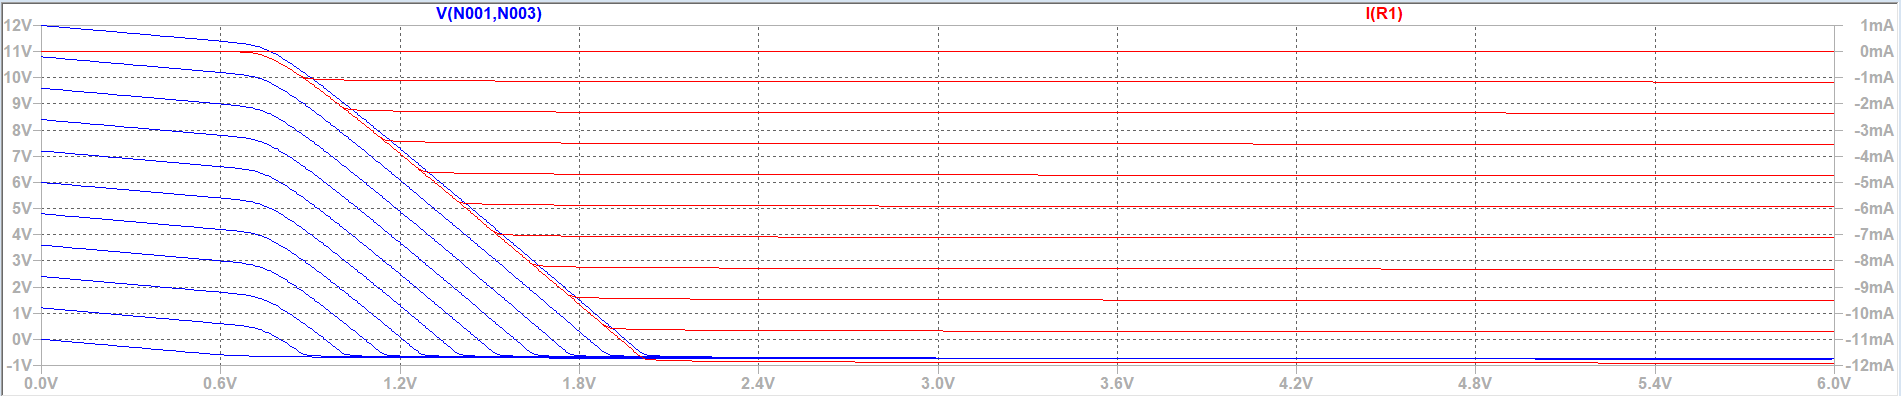
\includegraphics[width=1\textwidth]{7_c_plot.png}
\caption{Plot for step 7 d}
\end{figure} 


\section{Conclusion}
In this preliminary work document, some of the parameters of the different BJT's are examined. Then neccesssary simuloations concerning npn transistor characteristics are done and plotted. 

\section*{Appendix A}
The results of the some of the simulations are fetched from LTSpice and plotted in MATLAB in order to make the plots more readable and convenient.


\end{document}

%%%%%%%%%%%%%%%%%%%%%%   EXAMPLE TABLE   %%%%%%%%%%%%%%%%%%%%%%%%%%%%%%%%
\begin{table}[H]
\begin{center}
    \caption{Resistance reading by color code convention.}
    \vspace{2mm}
    \begin{tabular}{||c | c | c||} 
        \hline
        Color Order & Value & Tolerance \\ [0.5ex] 
        \hline\hline
        Brown / Black / Red / Gold & 1k\( \Omega \) & \( \% \) 5  \\ 
        \hline
        Yellow / Violet / Red / Gold & 4.7k\( \Omega \) & \( \% \) 5   \\
        \hline
        Brown / Grey / Orange / Gold & 18k\( \Omega \) & \( \% \) 5  \\ [1ex] 
        \hline
    \end{tabular}
\end{center}
\end{table}


%%%%%%%%%%%%%%%%%%%%%%   EXAMPLE IMAGE   %%%%%%%%%%%%%%%%%%%%%%%%%%%%%%%%
\begin{figure}[H]
\centering
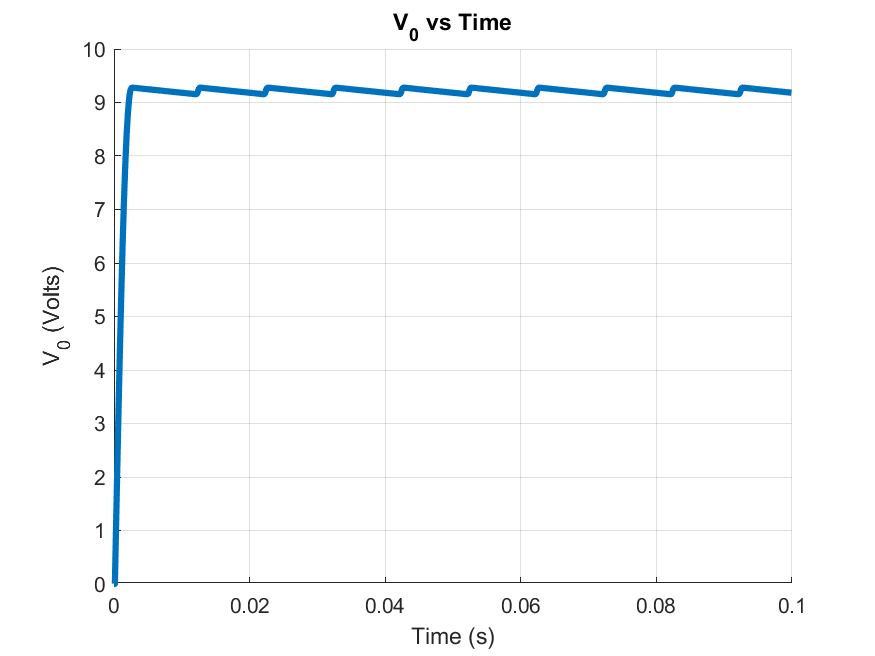
\includegraphics[width=1\textwidth]{5.png}
\caption{Circuit schematic for the step 5}
\end{figure} 

%%%%%%%%%%%%%%%%%%%%%%   EXAMPLE IMAGE FROM PDF   %%%%%%%%%%%%%%%%%%%%%%%%%%%%%%%%
\begin{figure}[H] \centering{
	\includegraphics[scale=0.25]{2a_plot.pdf}}
	\caption{Experiment 2}
\end{figure}
	